\documentclass[UTF8]{ctexart}
\usepackage{amsmath,amssymb}
\usepackage{fancyhdr}
\usepackage{amsmath,bm}
\usepackage{mathrsfs}
\usepackage{ntheorem}
\usepackage{graphicx}
\usepackage{subfigure}
\usepackage[top=2cm, bottom=2cm, left=2cm, right=2cm]{geometry}  
\usepackage{algorithm}  
\usepackage{algorithmicx}  
\usepackage{algpseudocode}
\usepackage{multirow}
\usepackage{tikz}
\usepackage{listings}
\usepackage{palatino}
\usepackage{xcolor}
\usepackage{syntax}
\usetikzlibrary{automata, positioning, arrows, shapes.geometric}
\tikzstyle{startstop} = [rectangle, minimum width = 2cm, minimum height=1cm,text centered, draw = black]
\tikzstyle{io} = [trapezium, trapezium left angle=70, trapezium right angle=110, minimum width=2cm, minimum height=1cm, text centered, draw=black]
\tikzstyle{process} = [rectangle, minimum width=3cm, minimum height=1cm, text centered, draw=black]
\tikzstyle{arrow} = [->,>=stealth]
\tikzstyle{decision} = [diamond, aspect = 3, text centered, draw=black]
\tikzset{
    ->,
    >=stealth,
    node distance = 3cm,
    every state/.style={thick, fill=gray!10},
    initial text=$ $
}
\lstset{numbers=left, %设置行号位置
        numberstyle=\tiny, %设置行号大小
        keywordstyle=\color{blue}, %设置关键字颜色
        commentstyle=\color[cmyk]{1,0,1,0}, %设置注释颜色
        frame=single, %设置边框格式
        escapeinside=``, %逃逸字符(1左面的键),用于显示中文
        %breaklines, %自动折行
        extendedchars=false, %解决代码跨页时,章节标题,页眉等汉字不显示的问题
        xleftmargin=2em,xrightmargin=2em, aboveskip=1em, %设置边距
        tabsize=4, %设置tab空格数
        showspaces=false %不显示空格
    }
\setlength{\grammarparsep}{10pt plus 1pt minus 1pt} % increase separation between rules
\setlength{\grammarindent}{20em} % increase separation between LHS/RHS 
\floatname{algorithm}{算法}  
\renewcommand{\algorithmicrequire}{\textbf{输入:}}  
\renewcommand{\algorithmicensure}{\textbf{输出:}}  

\theorembodyfont{\normalfont\rm\CJKfamily{song}}
%\theoremstyle{break}
\newtheorem{theorem}{定理}
\newtheorem{lemma}{引理}
\newtheorem{proposition}{命题}
\newtheorem*{proof}{证}[section]
\newtheorem*{solution}{解}[section]
\title{代码优化作业}
\author{丁元杰 17231164}
\date{\today}

\begin{document}
\maketitle

% 箭头形式

\section*{14.1}

流程图参见图\ref{sequence1}

\begin{figure}[htbp]
    \centering
        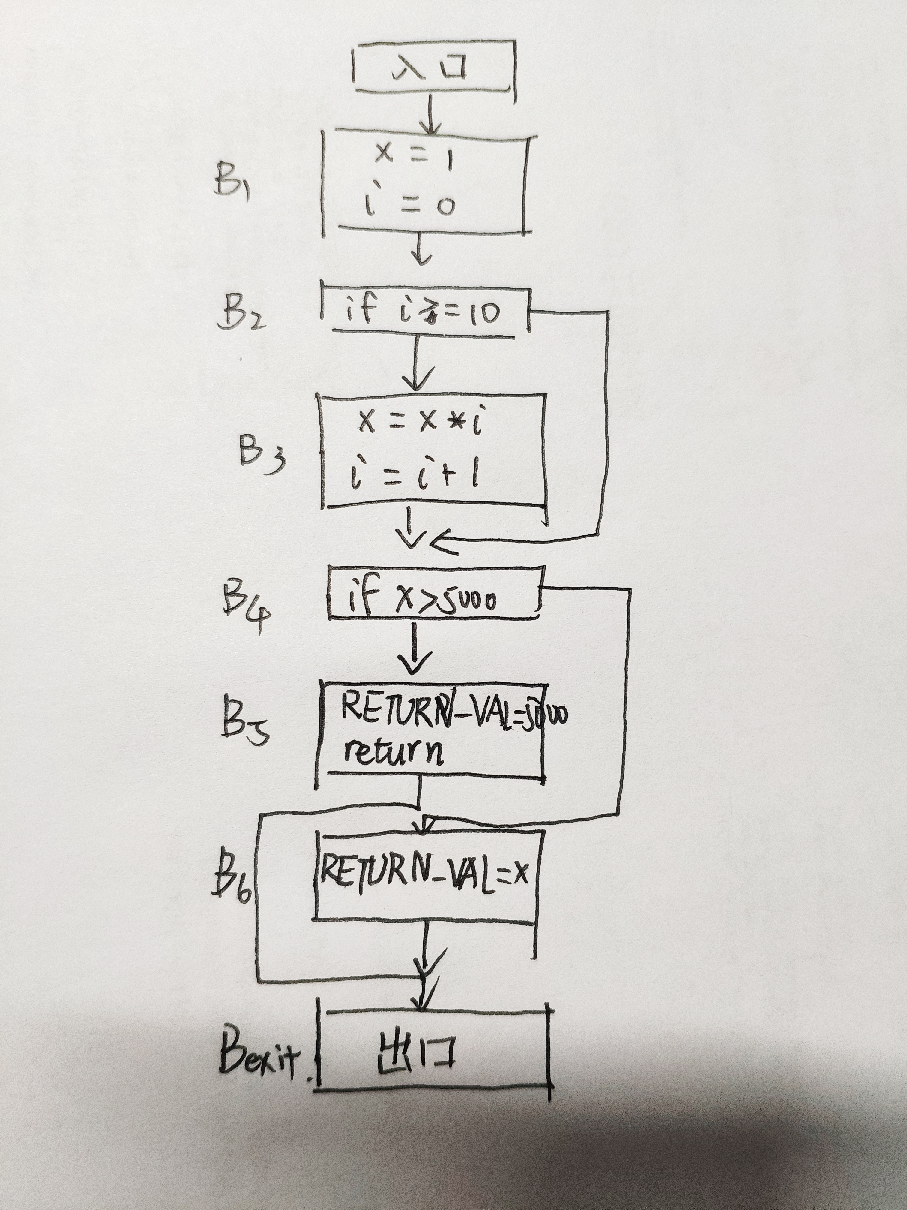
\includegraphics[width=5.5cm]{seqaq-small.png}
    \caption{第一题流程图}
    \label{sequence1}
\end{figure}

\section*{14.2}

转化过程请见图\ref{procedure}

\begin{figure}[htbp]
    \centering
    \subfigure[1]{
    \includegraphics[width=5.5cm]{seq1-small.png}
    %\caption{fig1}
    }
    \quad
    \subfigure[2]{
    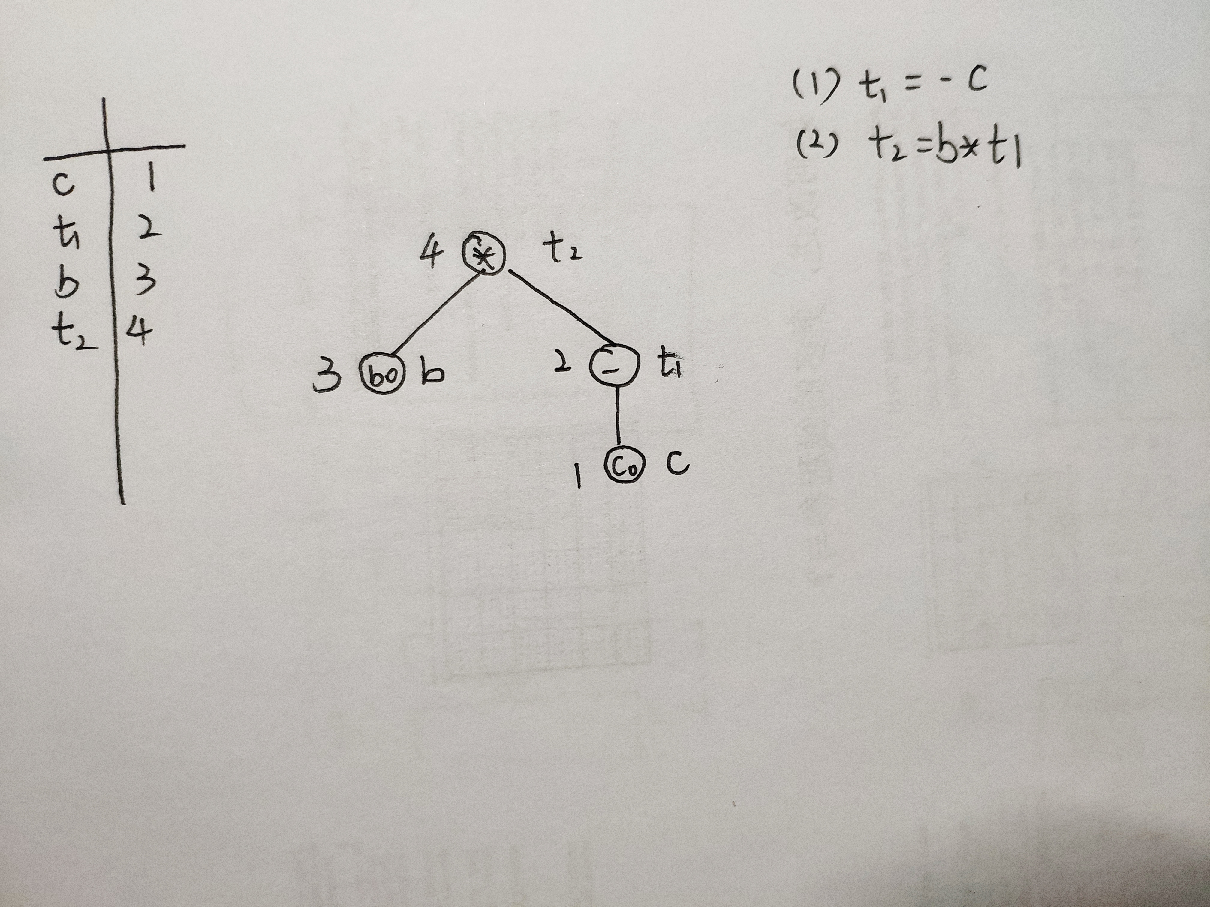
\includegraphics[width=5.5cm]{seq2-small.png}
    }
    \quad
    \subfigure[3]{
    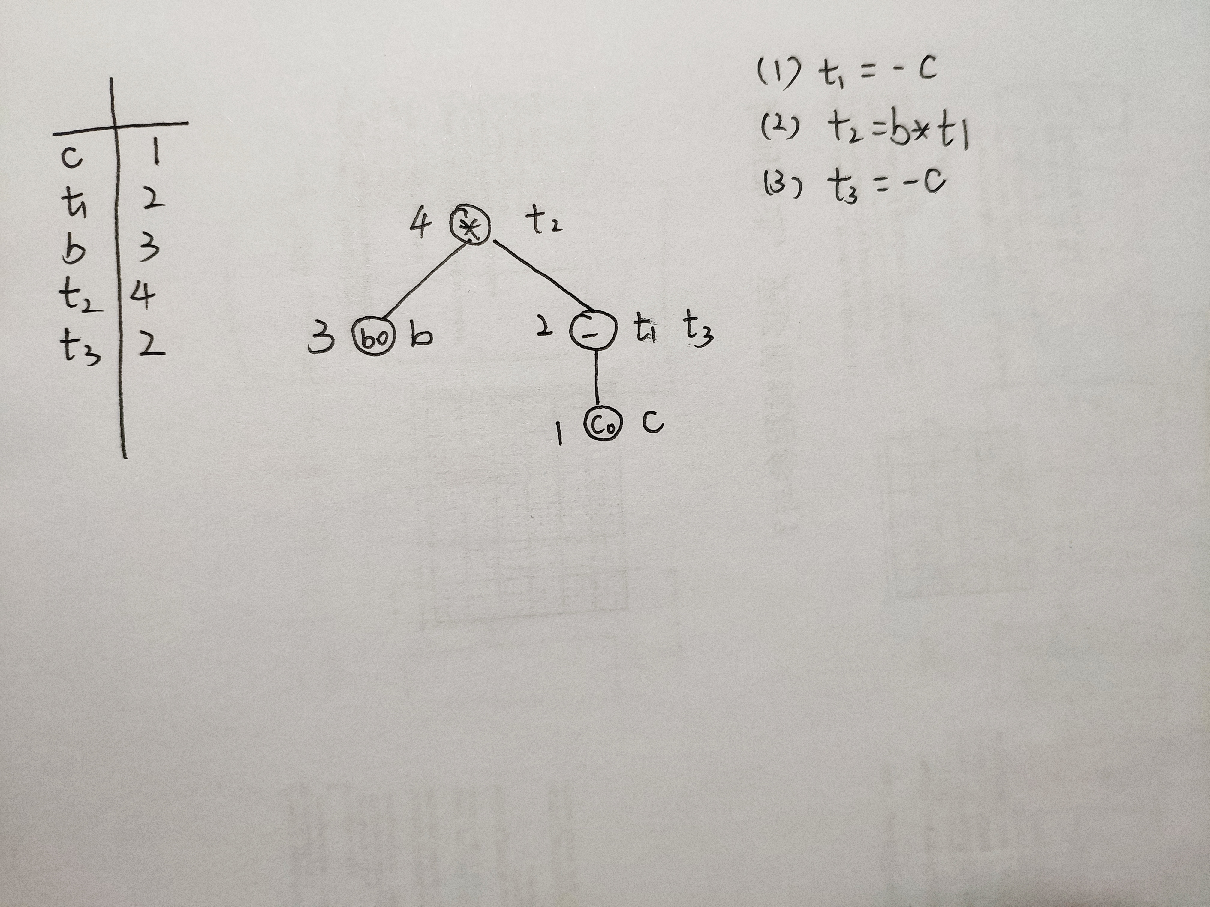
\includegraphics[width=5.5cm]{seq3-small.png}
    }
    \quad
    \subfigure[4]{
    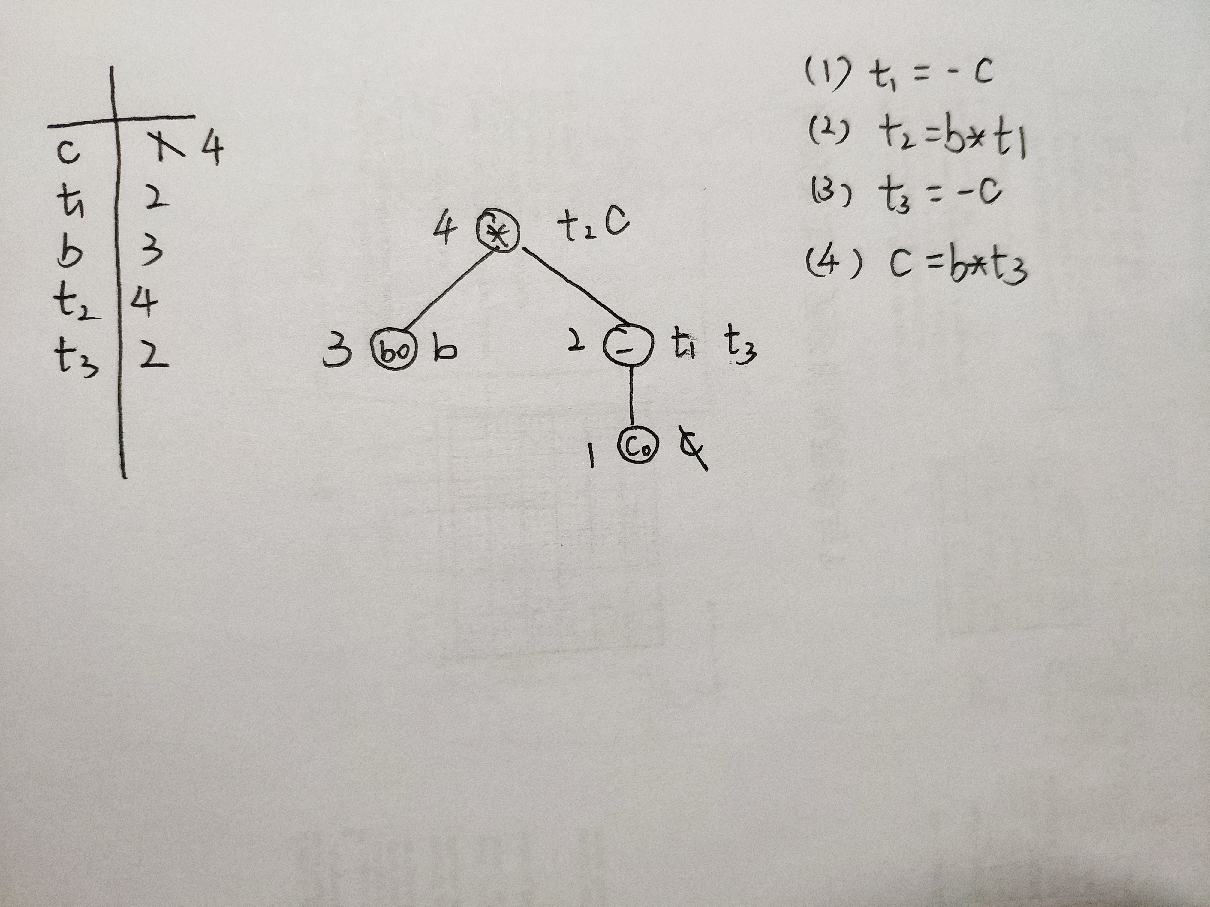
\includegraphics[width=5.5cm]{seq4-small.png}
    }
    \quad
    \subfigure[5]{
    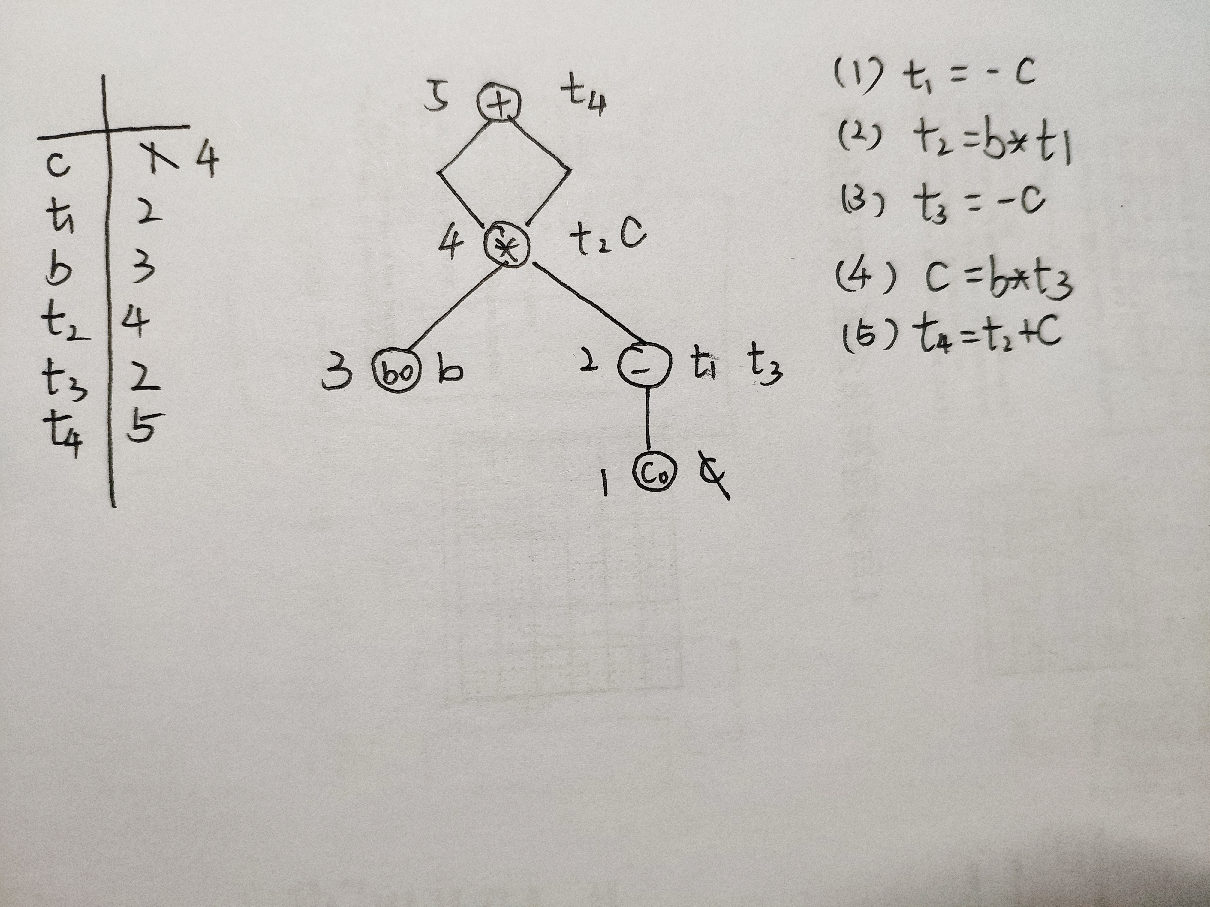
\includegraphics[width=5.5cm]{seq5-small.png}
    }
    \quad
    \subfigure[6]{
    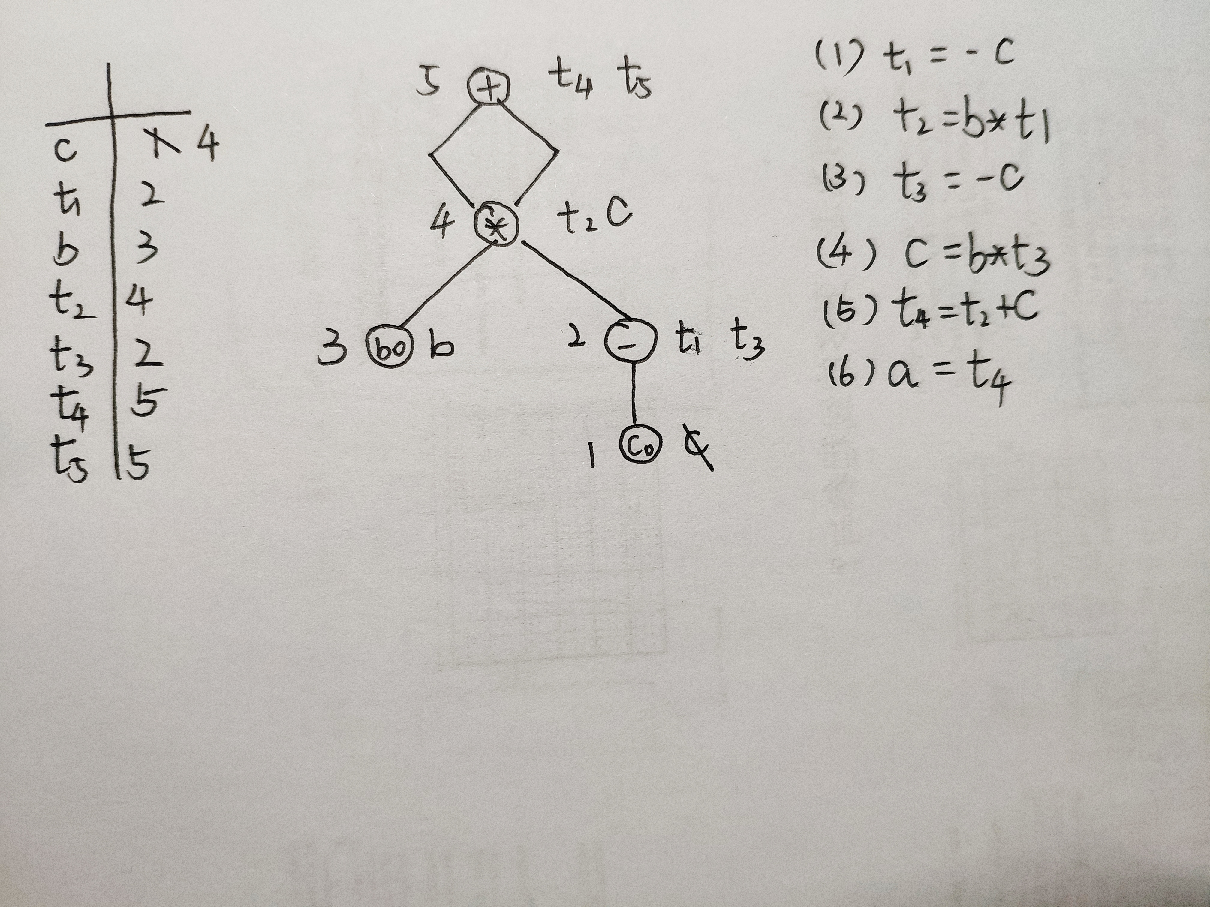
\includegraphics[width=5.5cm]{seq6-small.png}
    }
    \caption{转化过程}
    \label{procedure}
\end{figure}

\section*{14.3}

最终DAG和结点表如图\ref{dag};

\begin{figure}[htbp]
    \centering
        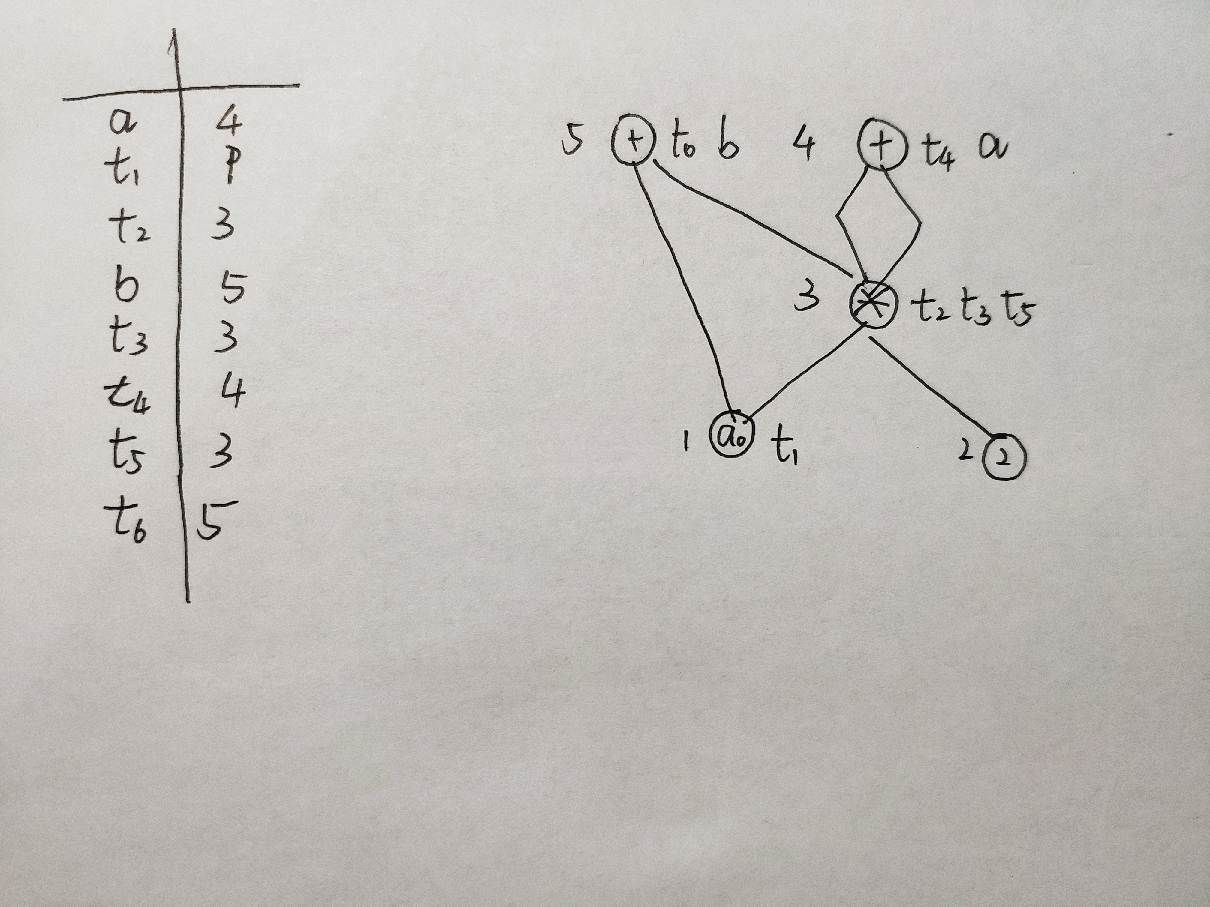
\includegraphics[width=5.5cm]{dag.png}
    \caption{第三题DAG}
    \label{dag}
\end{figure}

\end{document}